% Author @ Kurtik Appadoo, IN-PROGRESS, Reviewer @ Janak Subedi, Due Date 11/11
\subsection{Test Format}
All test files are structured using the mmi format, which is designed for representing graphs in a straightforward and consistent manner. The structure of the mmi format is detailed as follows:

\begin{itemize}
    \item The first line specifies the number of vertices in the graph, denoted as n.
    \item The second line indicates the number of partitions in the graph, referred to as d. A partition in this context is a set of vertices that only connect to vertices in other sets, not within the same set.
    \item The third line states the total number of edges or hyperedges in the graph, denoted as m. A hyperedge is a generalized edge that can connect more than two vertices, accommodating complex relationships in multi-dimensional graphs.
    \item The following m lines each represent a hyperedge in the graph, with each line containing d integers separated by spaces. These integers indicate the vertices connected by the hyperedge, ensuring connections between different partitions.
    \item The final line specifies the maximum matching in the graph, representing the maximum set of non-overlapping hyperedges where each vertex is included only once.
\end{itemize}

The mmi format is both simple and readable, making it highly suitable for generating large quantities of test cases efficiently while adhering to a standardized format. It is important to note that duplicate edges or hyperedges are not supported in this format, ensuring the uniqueness of connections within the graph.

\subsubsection{Storage and Naming Convention}
All mmi files are stored in their respective d directories within the test folder, organized by the number of partitions. Each file follows a strict naming convention to maintain clarity and consistency across the test suite:

\begin{verbatim}
    d{d}v{n}.mmi
\end{verbatim}

In this convention, d represents the number of partitions, and n indicates the number of vertices in each partition. This naming system allows for easy identification of the file contents without needing to open the file, promoting a standardized approach to organizing test cases.

\paragraph{Example}
\begin{figure}[h!]
    \centering
    \begin{minipage}{0.45\textwidth}
        \centering
        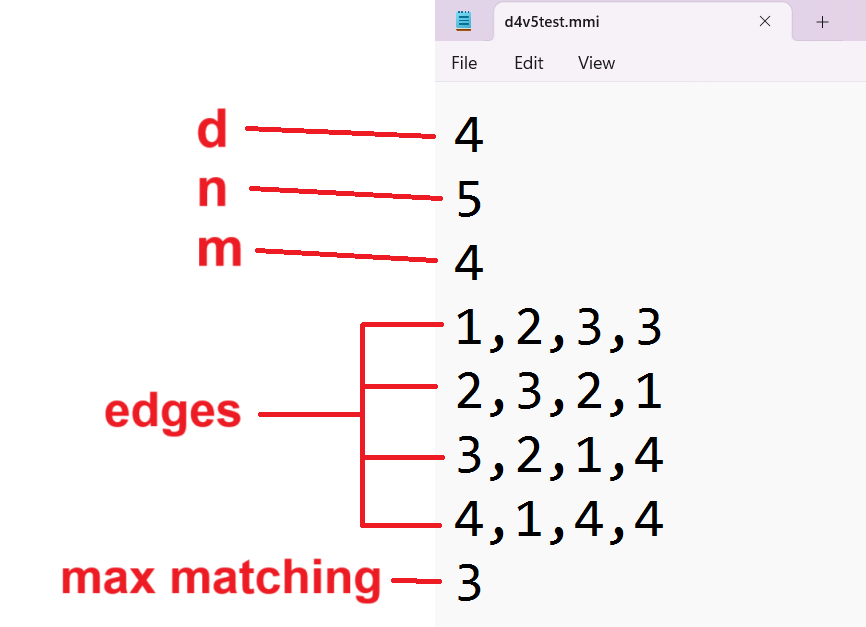
\includegraphics[width=\textwidth]{images/MMB_Solvers_Testing.png}
        \caption{An example of a test file in the mmi format.}
        \label{fig:image1}
    \end{minipage}
    \hfill
    \begin{minipage}{0.45\textwidth}
        \centering
        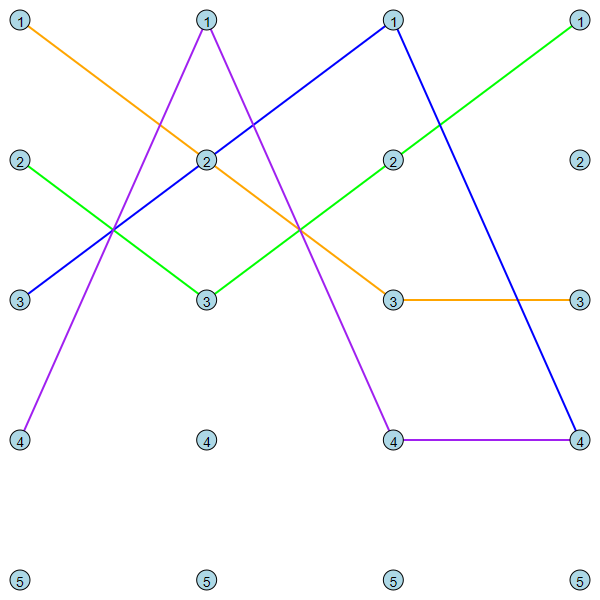
\includegraphics[width=\textwidth]{images/MMB_Solvers_Test.png}
        \caption{A visualization of the corresponding graph from Figure \ref{fig:image1}. The graph has 4 partitions, 5 vertices, and 4 hyperedges, with a maximum matching of 3 as indicated in the final line of the mmi file.}
        \label{fig:image2}
    \end{minipage}
\end{figure}

This format and naming convention provide a systematic and clear method for storing and referencing test cases, supporting efficient test generation and verification for maximum matching solvers in complex, multi-dimensional graph structures.